\lhead{\emph{Evaluation}}
\chapter{Evaluation}
\label{sec:evaluation}
% Intro
As mentioned in section [TODO: ref implementation section] the scope of the implementation in this thesis is limited to study the effects of exploring and navigating to music tracks. To study whether the Spatial Music Menu could compete with a touch and vision-based music player interface we designed and conducted an experiment where users should perform mental and physical demanding tasks while interacting with the interfaces.

TODO: Scope and limitations
- only using 1 gesture, we examined multiple gestures in pilot study (accuracy), too much noise in biking scenario: Unwanted activation of systems, too much learning, not important for measuring tasks

[TODO: rewrite]

- Only 5 participants, no statistical arguments but just hints
Regarding

- Possibly biased participants (friends) wants to perform good

- Limited measurement parameters e.g. not biking speed


\section{Experiment Design}
The experiment was designed and conducted as a controlled lab experiment. Controlled experiments are appropriate when comparing one design to another to see which is better \cite{benyon_designing_2010} and in this case we are compairing the Spatial Music Menu with a touch and vision-based music player. As the focus is on compairing and study the effects of these interfaces in an interaction in motion scenario i.e. biking, we designed a evaluation system simulating a trafficked biking scenario.

\subsection{Biking simulation setup}
A stationary bike was put in front of a giant screen (4 x 40 inch HD screens) that should simulate a road. To make the view as realistic as possible an image of an actual trafficked road\footnote{New York street: \url{http://timsklyarov.com/new-york-through-the-eyes-of-a-road-bicycle/}} was showed on the screen. To simulate obstacles that the user should be aware of or respond to in a real world biking scenario, 3 different shapes with random colors were displayed in random positions on the screen in a random time interval; between 0.3 and 1 second displaying the shape in 0.8 seconds. The shapes were circles, triangles and squares and the job for the person riding the bike was to detect the circles. This was done by pushing a button attached close to the users non-preferred hand on the steer, in this case a Playstation 3 joystick strapped with tape. The reason for the button placement at the non-preferred hand was, that the preferred hand should be used for navigating the touch and vision-based music player. To give the user feedback the circle was removed when detected. The screen simulation software is developed in Python 3 running on a Mac (OSX 10.9). The simulation system is illustrated in figure [TODO: ref].

[TODO: figure of biking simulation system]

\subsection{Touch and vision-based music player}
To represent a touch and vision-based music player we chose the music streaming service Deezer\footnote{\url{https://www.deezer.com/}}. Their Android application\footnote{\url{https://play.google.com/store/apps/details?id=deezer.android.app}} was installed on a Google Nexus 4 running Android 4.3. The same headset as for the Spatial Music Menu was used but this time connected through a wire.

\subsection{Hypotheses}
Based on the related work theory behind the design choices for the Spatial Music Menu we derived the following hypotheses for the experiment:

\begin{description}
\item[Hypothesis 1:] The users ability to detect circles while executing tasks in the biking simulation will increase with the Spatial Music Menu interface compaired to the touch and vision-based music player interface.
\end{description}

\begin{description}
\item[Hypothesis 2:] The users performance when executing tasks in the biking simulation using the Spatial Music Menu can compete with the touch and vision-based music player interface in terms of general usability (workload).
\end{description}


\section{Method}
[TODO: intro]

\section{Participants}
5 persons (all male) were chosen for the evaluation. They all have in common that they listens to music while biking regurarly. The participants had an average age of 30 years.

\subsection{Procedure}
[TODO: instructions, preparation, favourite tracks]
% Prerequisites
... before starting the experiment the user were instructed in how the Spatial Music Menu works i.e. which head gestures to use for navigating and how the menu structure looks. They then got a chance to try out the system both standing still and while riding the stationary bike. In the standing still scenario the user was allowed to look at the menu envisioned on the iPad screen to get a sense of the menu structure and interaction feedback...

% Task description
[TODO: Task description]

- Artist - Album - Track

- task traditional: Pick phone from pocket, activate, navigate, deactivate, back in pocket

- choosing music tracks in Deezer app

User performing a task using the Spatial Music Menu is shown in figure \ref{fig:evalspatial}

\begin{figure}[t]
	\centering
		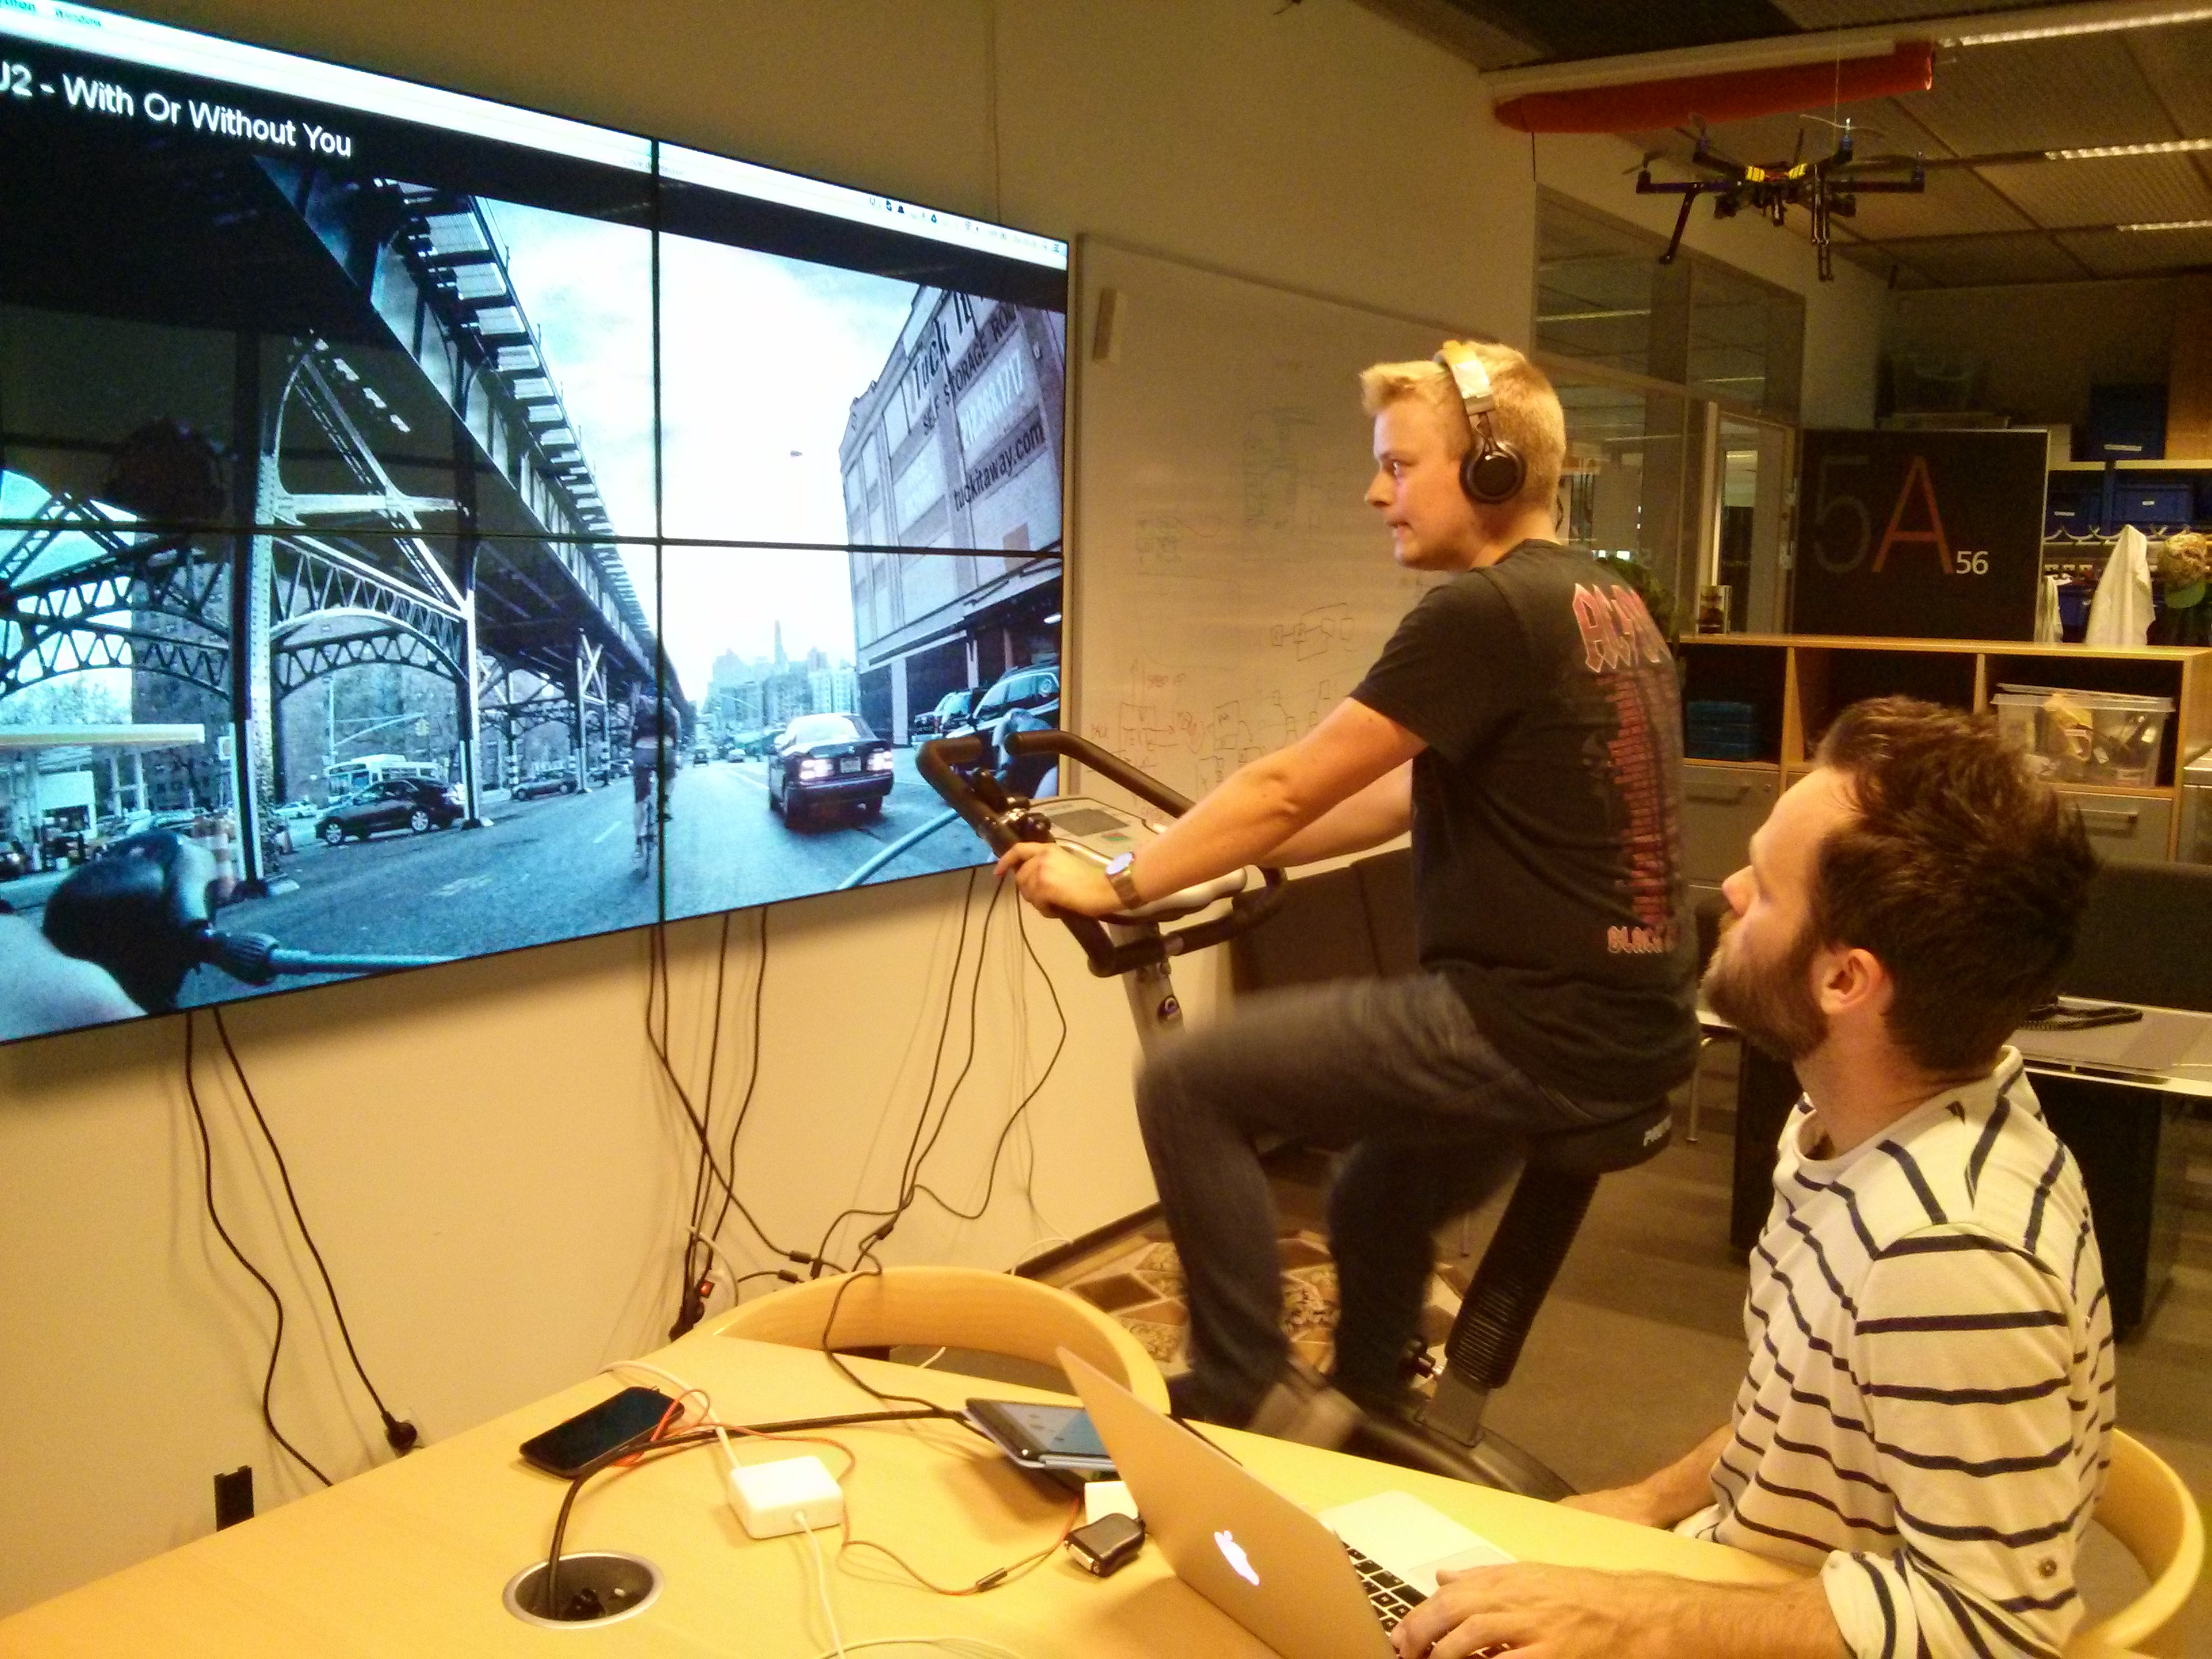
\includegraphics[width=0.7\textwidth,height=\textheight,keepaspectratio]{./Figures/evaluation_spatial.jpg}
		\rule{35em}{1pt}
	\caption[Evaluation Spatial Music Menu]{Participant performing a task using the Spatial Music Menu}
	\label{fig:evalspatial}
\end{figure}

User performing a task using a touch and vision-based music player is shown in figure \ref{fig:evalspatial}

\begin{figure}[t]
	\centering
		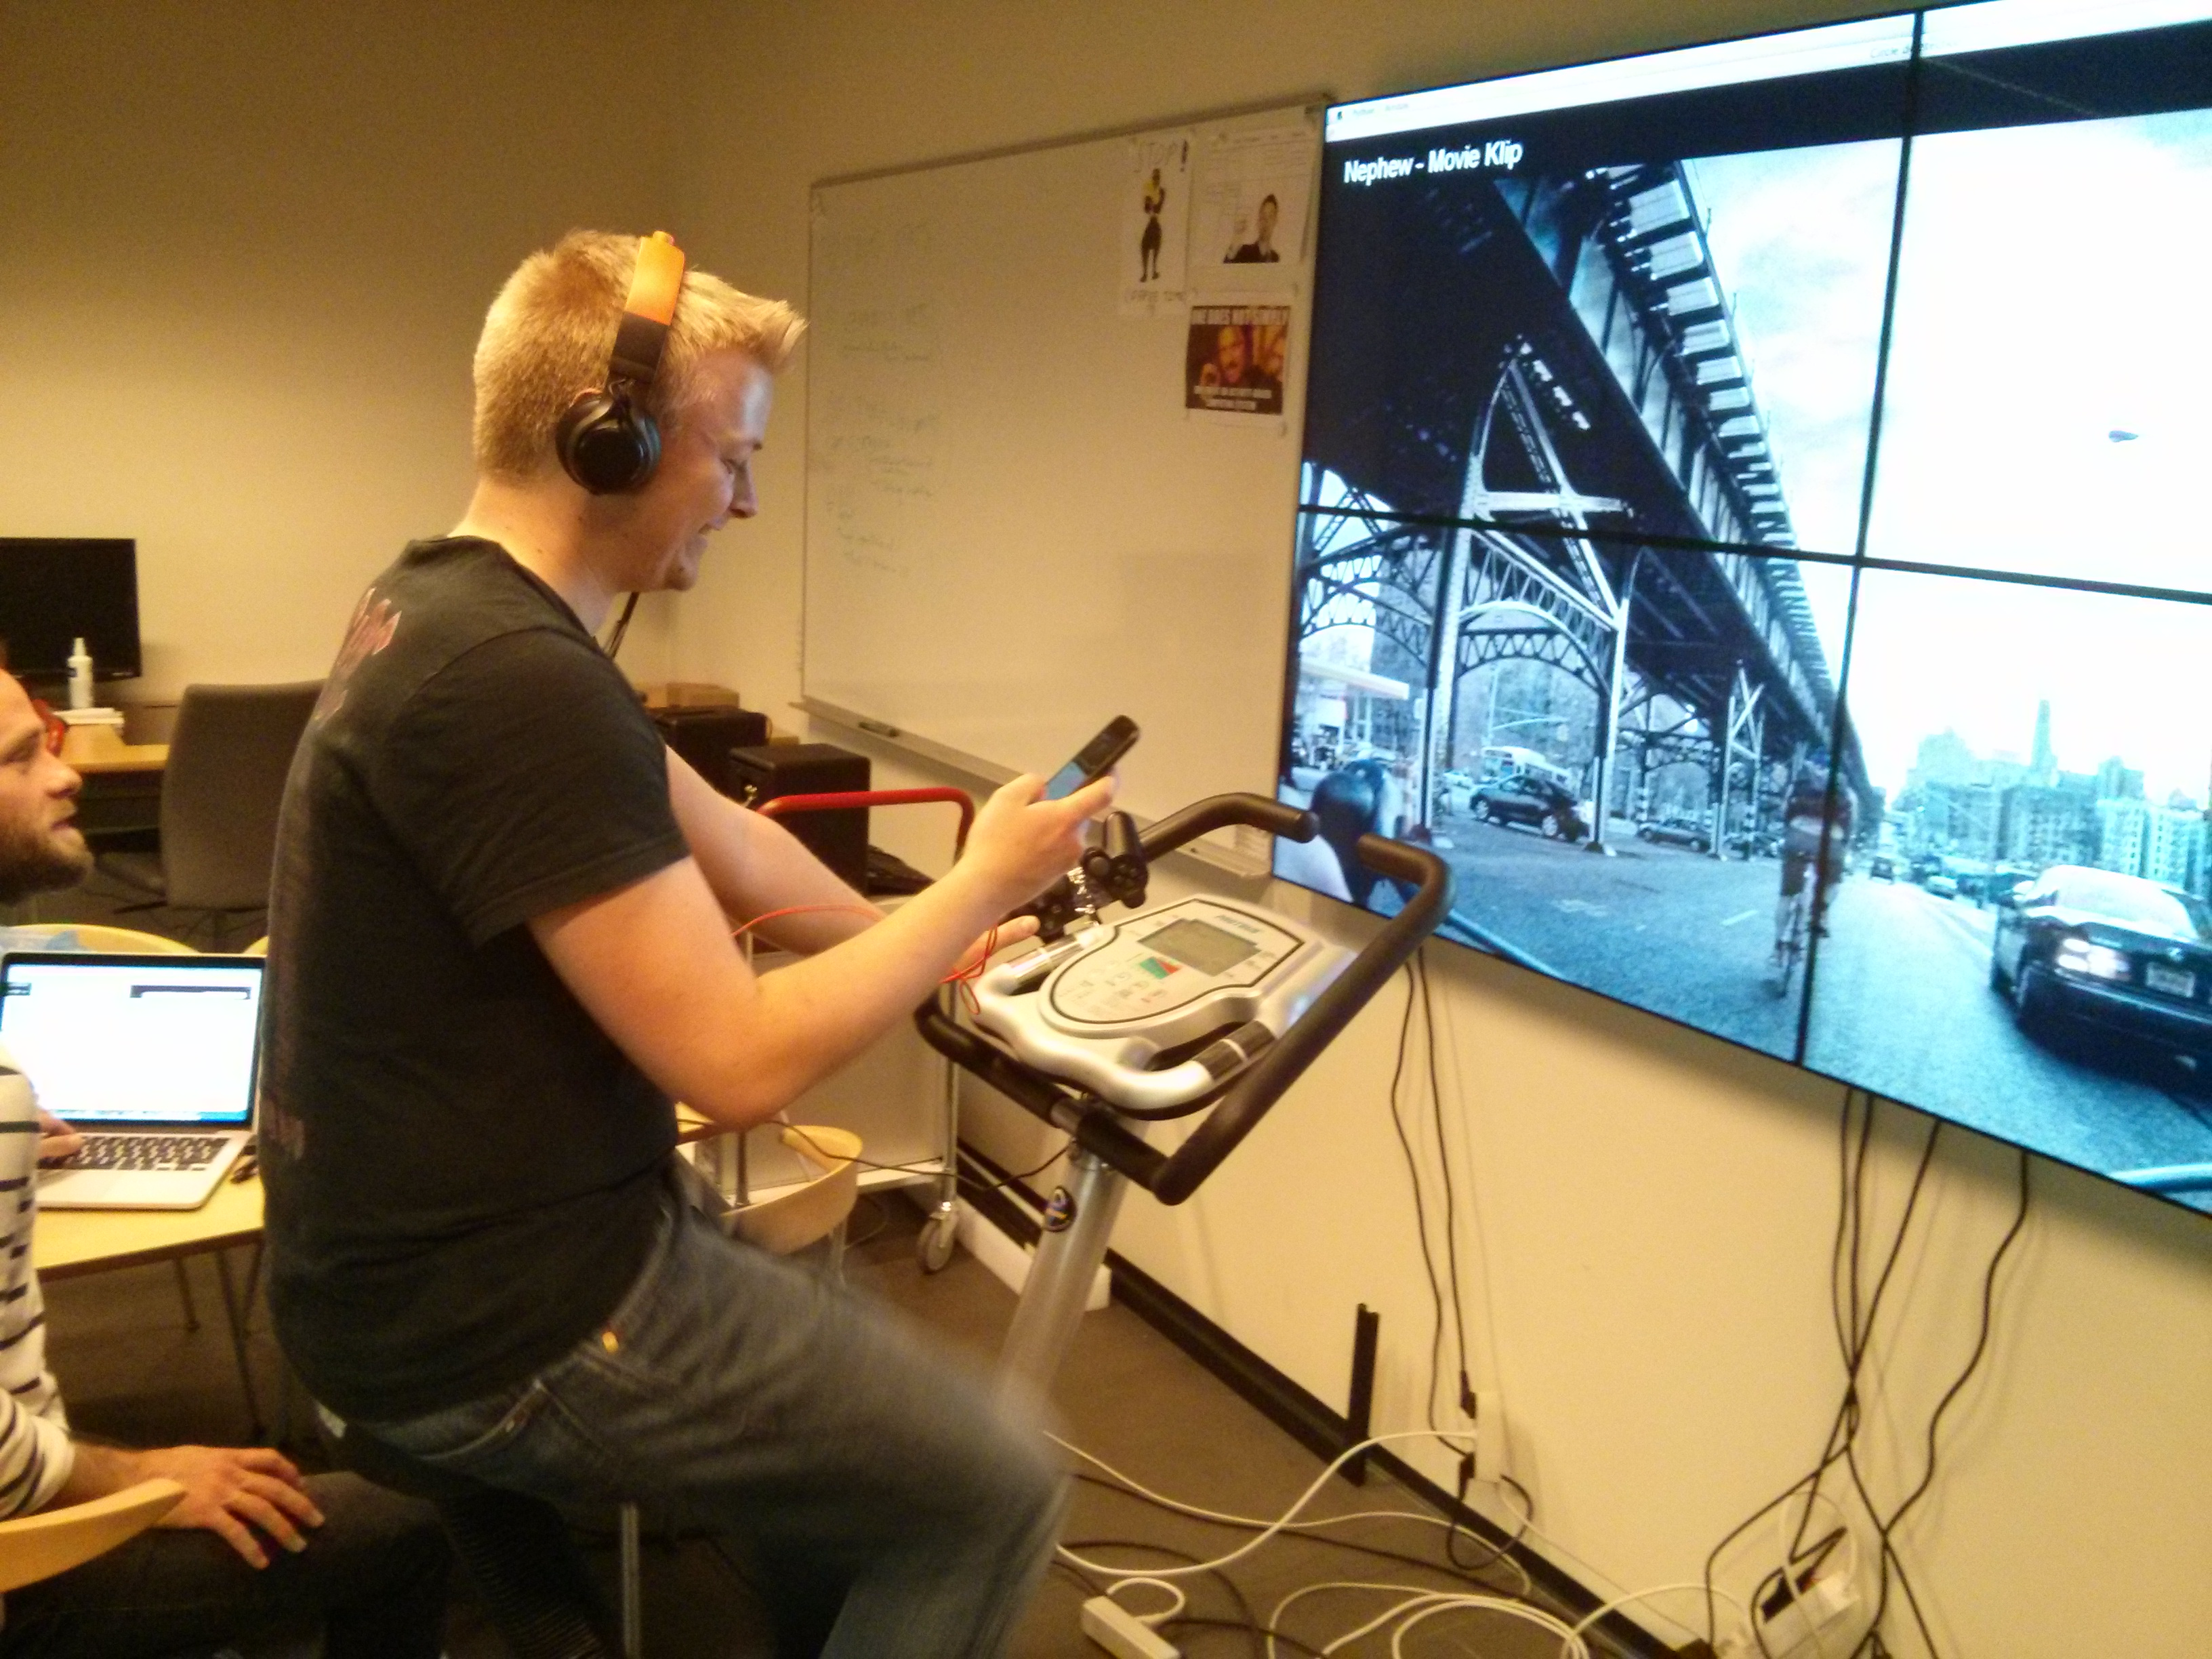
\includegraphics[width=0.7\textwidth,height=\textheight,keepaspectratio]{./Figures/evaluation_normal.jpg}
		\rule{35em}{1pt}
	\caption[Evaluation touch and vision-based interface]{Participant performing a task using a touch and vision-based music player}
	\label{fig:evalspatial}
\end{figure}

\subsection{Logging}
Throughout the experiment several data were logged. This includes data from the Biking Simulation System: Task start/end, circles shown, circles detections, error detections - and data from the Spatial Music Menu: Gestures detected, navigation steps including track info, headset connection status. Every log subject has a timestamp and as logging were performed on two different systems - iOS and OSX (python script) clocks were synchronized before comparison.


\subsection{NASA Task Load Index}
Subjective workload was measured using the NASA Task Load Index (TLX) scales \cite{hart_workload_1990}. The scales includes mental demand, physical demand, temporal demand, performance, effort and frustration in which each participant should rate after testing. The user ratings gives a qualitative analysis of the system and the perceived workload is linked with the general usability of the system.

\subsection{Observing and semi-structured interview}

- Monitoring interaction via iPad screen, calibrating center direction

- General user feedback at the end of tests


\section{Results}
[TODO: intro]

\subsection{User performance}
[TODO]
% Number of circles, safety
%The most important task for the user during testing is to detect as many circles as possible. The number of circles shown and the number of circles detected were logged during execution of tasks. This will give a quantitative analysis of whether the user is able to monitor the surroundings while interacting with the systems and contribute to the safety problem focus.

% System, track exploring
%For measuring the content (music track) exploring part of the Spatial Music Menu all navigation information were logged on the iPad. 

% System, task time

Circles detected, figure \ref{fig:resultscircles}

\begin{figure}[t]
	\centering
		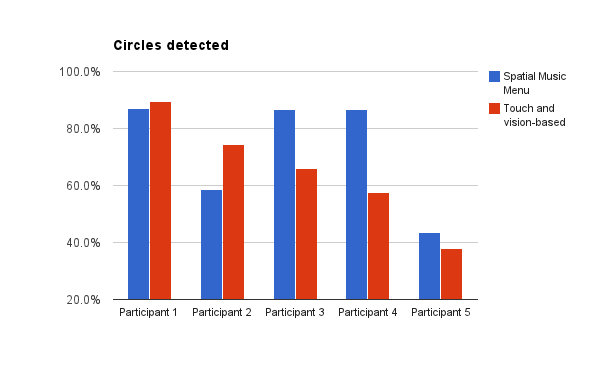
\includegraphics[width=0.9\textwidth,height=\textheight,keepaspectratio]{./Figures/results_circles.png}
		\rule{35em}{1pt}
	\caption[Results circle detections]{Percentage of circles detected for the participants}
	\label{fig:resultscircles}
\end{figure}


Task time execution, figure \ref{fig:resultstasktime}

\begin{figure}[t]
	\centering
		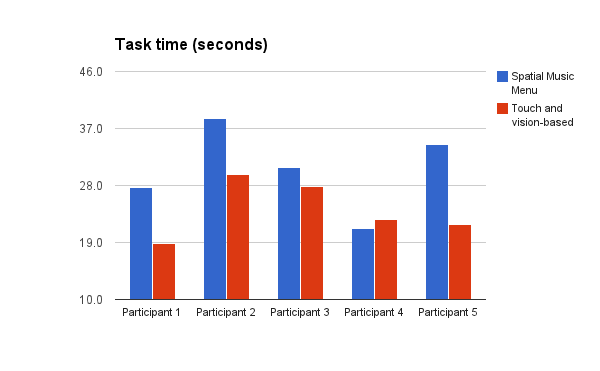
\includegraphics[width=0.9\textwidth,height=\textheight,keepaspectratio]{./Figures/results_task_time.png}
		\rule{35em}{1pt}
	\caption[Results task time]{Time taken (in seconds) in average to execute a task for the participants}
	\label{fig:resultstasktime}
\end{figure}

\subsection{Workload}
[TODO]

... it can give an indication of how much of the users physical and mental resources is required by the system during interaction and thereby an indication of the resources left for monitoring and navigating the surroundings when biking i.e. a safety parameter.

Nasa TLX scores, figure \ref{fig:resultsnasatlx}

\begin{figure}[t]
	\centering
		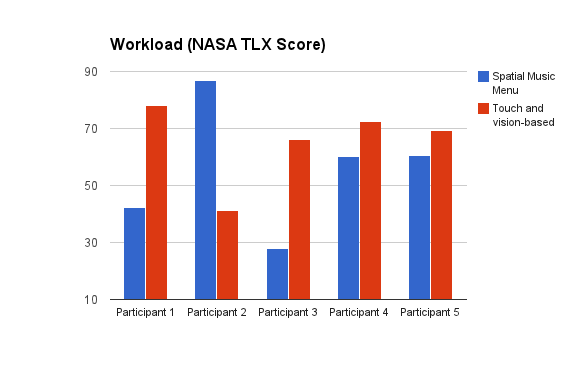
\includegraphics[width=0.9\textwidth,height=\textheight,keepaspectratio]{./Figures/results_nasatlx.png}
		\rule{35em}{1pt}
	\caption[Results NASA TLX Score]{NASA TLX overall workload score for the participants (less is better)}
	\label{fig:resultsnasatlx}
\end{figure}

\subsection{Discussion}
...

Challenges:\\
- Spatial sound through headphones depend on the HRTF recorded and might not fit to all persons as the ear constructions are different (Brewster chapter 12 "Non-Speech Auditory Output" \cite{brewster_human-computer_2003})





% Maybe comfort as a measurement?
%(Taken from Brewster article)
%The final measure taken was comfort. This was based around a new scale developed by Knight et al. [10] called the Comfort Rating Scale (CRS) which assesses various aspects to do with the comfort of a wearable device. For a device to be accepted and used it needs to be comfortable and people need to be happy to wear it. Using a range of 20- point rating scales similar to NASA TLX, CRS breaks com- fort into 6 categories: emotion, attachment, harm, perceived change, movement and anxiety. Knight et al. have used it to assess the comfort of two wearable devices they are building in their research group. Using this will allow us to find out more about the actual acceptability our systems.



